\section{Protocolo HTTP}

El Protocolo de transferencia de hipertexto (HTTP) es un protocolo de 
solicitud/respuesta \emph{stateless} (sin estado) que utiliza semántica 
extensible y cargas útiles de mensajes autodescriptivos para una 
interacción flexible con sistemas basados en red.

   HTTP es un protocolo genérico para sistemas de información. Está 
   diseñado para ocultar los detalles de cómo se implementa un servicio 
   mostrando una interfaz a los clientes que es independiente de los 
   tipos de recursos proporcionados. Del mismo modo, los servidores 
   no necesitan conocer el propósito de cada cliente: una solicitud 
   HTTP puede aislada en vez de estar asociada con un tipo específico
    de cliente o una secuencia predeterminada de pasos de la aplicación.
     
    El resultado es un protocolo que se puede utilizar de forma eficaz 
     en muchos contextos diferentes y cuyas implementaciones pueden
      evolucionar a lo largo del tiempo.
   Una consecuencia de esta flexibilidad es que el protocolo no 
   se puede definir en términos de lo que ocurre detrás de la 
   interfaz: estamos limitados a definir la sintaxis de la comunicación, 
   los mensajes y el comportamiento esperado de los destinatarios. 
   Si la comunicación se considera de forma aislada, las acciones 
   exitosas deben reflejarse correspondientemente. Sin embargo, 
   dado que varios clientes pueden actuar en paralelo y quizás con
    propósitos cruzados, no podemos exigir que tales cambios sean 
    observables más allá del alcance de una única respuesta.
   
\subsection{Arquitectura}
HTTP fue creado para la arquitectura World Wide Web (WWW) y ha 
evolucionado con el tiempo para soportar las necesidades de
 escalabilidad de un sistema mundial. Gran parte de esa arquitectura 
 se refleja en la terminología y  definiciones de sintaxis utilizadas 
 para definir HTTP.

\subsubsection*{Mensajes Cliente/Servidor}


HTTP es un protocolo de solicitud/respuesta que opera intercambiando 
mensajes a través de una ``conexión'' en la capa de sesión o transporte.
 Un “cliente” HTTP es un programa que establece una conexión a un 
 servidor con el propósito de enviar una o más solicitudes HTTP. 
 Un “servidor” HTTP es un programa que acepta conexiones para
  atender solicitudes HTTP mediante el envío de respuestas HTTP. 
  La mayoría de las comunicaciones HTTP consisten en una solicitud
   (GET) de algún recurso identificado por un URI. En el caso más 
   simple, esto podría lograrse mediante una única conexión entre un
    usuario y el servidor.

\begin{center}
   \begin{figure}   
      \begin{center}
         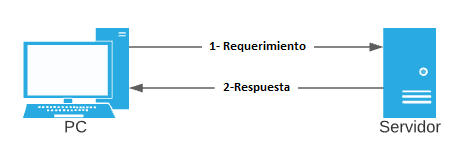
\includegraphics{2.1.png}
      \end{center}
      \caption{Comunicación básica en HTTP}
   \end{figure}
\end{center}

Un cliente envía una solicitud HTTP a un servidor en forma de mensaje
 de solicitud, comenzando con una línea que incluye un método, URI y 
 versión del protocolo, seguida de campos de encabezado que contienen
  modificadores de solicitud, información del cliente y metadatos de
   representación, una línea vacía para indicar el final de la sección
    del encabezado, y finalmente un cuerpo del mensaje que contiene el 
    cuerpo de la carga útil (si lo hay). 
    
    Un servidor responde a la 
    solicitud de un cliente enviando uno o más mensajes de respuesta 
    HTTP, cada uno de los cuales comienza con una línea de estado que 
    incluye la versión del protocolo, un código de estado (éxito o error)
     y una descripción en forma de texto asociada al mismo, posiblemente 
     seguida de campos de encabezado con información del servidor y
      metadatos de recursos, una línea vacía para indicar el final 
      de la sección del encabezado y finalmente, un cuerpo del mensaje
       la carga útil del mismo

\subsubsection*{Ejemplo}
El siguiente ejemplo ilustra un intercambio de mensajes típico 
para una solicitud GET a la dirección “http://www.example.com/hello.txt”:

\bigskip
\noindent
\underline{Client request:}
\begin{verbatim}
   GET /hello.txt HTTP/1.1
   User-Agent: curl/7.16.3 libcurl/7.16.3 OpenSSL/0.9.7l zlib/1.2.3
   Host: www.example.com
   Accept-Language: en, mi
  \end{verbatim}
\underline{Server response:}
\begin{verbatim}
   HTTP/1.1 200 OK
   Date: Mon, 27 Jul 2009 12:28:53 GMT
   Server: Apache
   Last-Modified: Wed, 22 Jul 2009 19:15:56 GMT
   ETag: "34aa387-d-1568eb00"
   Accept-Ranges: bytes
   Content-Length: 51
   Vary: Accept-Encoding
   Content-Type: text/plain

   Hello World! My payload includes a trailing CRLF.
\end{verbatim}


\subsection{Métodos mas importantes del del protocolo HTTP}

El protocolo HTTP contiene varios métodos, como por ejemplo PUT, HEAD, DELETE, etc. Sin
embargo, para nuestro trabajo explicaremos los dos mas utilizados GET y POST, lo que
nos permitirá tener una base a la hora de presentar el caso de estudio de la 
sección \ref{secCaseOfStudy}.

%CONNECT OPTIONS TRACE PUT 

\subsubsection*{GET}

El método GET solicita al servidor la transferencia de un recurso.
GET es el mecanismo principal de recuperación de información y el 
foco de casi todas las optimizaciones de rendimiento. Por lo tanto,
cuando las personas hablan de recuperar información identificable
a través de HTTP, generalmente se refieren a realizar una solicitud
GET.

Se puede pensar que a la hora de solicitar un recuro, este sea un archivo 
dentro de un directorio, y la respuesta sea el mismo archivo. Sin embargo, 
no existen tales limitaciones en la práctica. De hecho, se puede 
configurar un servidor para ejecutar los archivos de la solicitud y 
enviar la salida en lugar de transferir los archivos directamente. 
Independientemente de la solicitud, el servidor solo necesita saber 
cómo tratar a cada uno de sus recursos.

\subsubsection*{POST}

El método POST solicita que un recurso del servidor sea procesado con 
los datos que el cliente le envía. Por ejemplo, POST se utiliza para 
las siguientes funciones (entre otras):

\begin{itemize}
   \setlength\itemsep{-0.6em}
   \item Proporcionar un bloque de datos, como los campos ingresados 
   en un formulario HTML, a un proceso de manejo de datos.
   \item Publicar un mensaje grupo de 
   noticias, lista de correo, blog o grupo similar de artículos.
   \item Crear un nuevo recurso que aún no ha sido identificado por 
   el servidor.
   \item Agregar datos a las representaciones existentes de un recurso.
\end{itemize}


\subsection{Códigos de respuesta} 
El código de estado es un número entero de tres dígitos que da el 
resultado del intento de comprender y satisfacer la solicitud.
   Los códigos de estado HTTP son extensibles. No se requiere que los
    clientes HTTP comprendan el significado de todos los códigos de
     estado registrados, aunque se espera una mínima comprensión.

   Por ejemplo, si un cliente recibe un código de estado no reconocido
    de 471, el cliente puede asumir que hubo algo mal con su solicitud
     y tratar la respuesta como si hubiera recibido un código de estado
      400 (Solicitud incorrecta). El mensaje de respuesta generalmente 
      contendrá una representación que explica el estado.

   El primer dígito del código de estado define la clase de respuesta.
    Los dos últimos dígitos no tienen ninguna función de categorización.
     Hay cinco valores para el primer dígito:

   \begin{itemize}
      \setlength\itemsep{-0.6em}
      \item 1xx (Informativo): Se recibió la solicitud, se continua procesando.
      \item 2xx (Satisfactoria): La solicitud se recibió, comprendió y 
      aceptó correctamente.
      \item 3xx (Redireccionamiento): Se deben realizar más acciones para
    completar la solicitud.
    \item 4xx (Error del cliente): La solicitud contiene una sintaxis
    incorrecta o no se puede cumplir.
    \item 5xx (Error del servidor): El servidor no cumplió con una
       solicitud aparentemente válida.
   \end{itemize}

\subsection{Infraestructura de clave pública: una Introducción a la navegación segura (EL CONTENIDO 
VA A SER AGREGADO DESPUES DEL PRIMER FEEDBACK) }   

%
Gracias a la criptografía de clave pública, podemos comunicarnos de forma 
segura y confidencial con 
las personas cuyas claves públicas tengamos, pero hay una serie de problemas 
que siguen sin resolverse. Por ejemplo, ¿cómo podemos comunicarnos con personas que 
nunca hemos conocido? ¿Cómo almacenamos las claves públicas y las revocamos? Más 
importante aún, ¿cómo lo hacemos a escala mundial, con millones de servidores y 
miles de millones de personas y dispositivos? Es una tarea difícil, pero para eso 
se creó la infraestructura de clave pública (PKI).

El objetivo de PKI es permitir una comunicación segura entre partes que nunca se 
han conocido antes. El modelo que usamos hoy se basa en “trusted third parties” 
llamados autoridades de certificación (\emph{CA}, a veces también llamadas autoridades 
de certificación) para emitir certificados en los que confiamos siempre. Una 
infraestructura PKI está formado por los siguientes agentes.


\subsubsection*{Suscriptor}


El suscriptor (o entidad final) es la parte que desea brindar servicios 
seguros, que requieren un certificado. Por ejemplo: una empresa que desea 
publicar su sitio web.

\subsubsection*{Autoridad de Registro}

La autoridad de registro (RA) lleva a cabo determinadas funciones de gestión 
relacionadas con la emisión de certificados. Por ejemplo, una RA puede realizar 
la validación de identidad necesaria antes de solicitar a una \emph{CA} que emita un 
certificado. En algunos casos, las RA también se denominan autoridades de 
registro local (LRA). En la práctica, muchas \emph{CA} también realizan tareas de RA.

\subsubsection*{Autoridad de certificación}

Una autoridad de certificación (\emph{CA}) es un agente en el que confiamos para emitir 
certificados que confirman las identidades de los suscriptores. También están 
obligados a proporcionar información de revocación actualizada en línea para 
que las partes que confían puedan verificar que los certificados siguen siendo válidos.

\subsubsection*{Consumidor de certificados}

Técnicamente, se trata de los navegadores web, de programas y de sistemas 
operativos que realizan la validación de certificados. Para ello, contienen 
almacenes que contienen los certificados de confianza de algunas \emph{CA}. En un 
sentido más amplio, los agentes que confían son los usuarios finales que 
dependen de certificados para una comunicación segura en Internet.

\subsubsection*{Certificados}

Un certificado es un documento digital que contiene una clave pública, cierta 
información sobre la entidad asociada y una firma digital del emisor del 
certificado. En otras palabras, es una herramienta que nos permite intercambiar, 
almacenar y usar claves públicas. Con eso, los certificados se convierten en 
el componente básico de PKI.

\subsubsection*{Cadenas de certificados}

En la mayoría de los casos, un certificado de una entidad final por sí solo es 
insuficiente para una validación exitosa. En la práctica, cada servidor debe 
proporcionar una cadena de certificados que conduzca a una raíz de confianza. 
Las cadenas de certificados se utilizan por motivos de seguridad, técnicos y 
administrativos.

\subsubsection*{Autoridades de certificación}

Las autoridades de certificación (\emph{CA}) son la parte más importante del modelo 
actual de confianza en Internet. Pueden emitir un certificado para cualquier 
nombre de dominio, lo que significa que todo lo que digan es válido. 
Durante mucho tiempo, el costo de los certificados era bastante elevado. 
Sin embargo, en estos días, el precio se redujo drásticamente, impulsado 
por una fuerte competencia, adicionando a varias organizaciones que proveen 
estos servicios de manera gratuita. 

\subsubsection*{Ciclo de vida del certificado}

El ciclo de vida del certificado comienza cuando un suscriptor prepara una 
Solicitud de firma de certificado (CSR) y la envía a la \emph{CA} de su elección. 
El propósito principal del CSR es poner a disposición de la \emph{CA} la clave 
pública, así como demostrar la propiedad de la clave privada correspondiente 
(mediante una firma). 


\begin{center}
    \begin{figure}   
       \begin{center}
          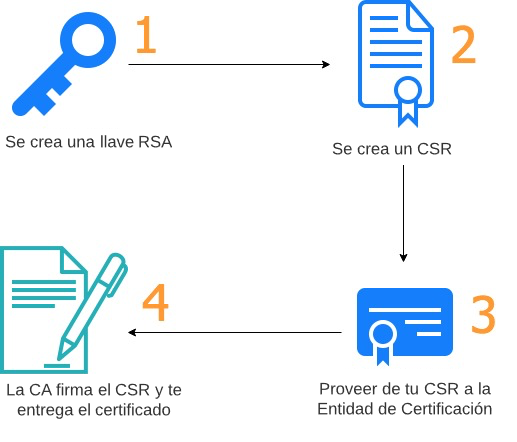
\includegraphics[width=9cm,height=8cm]{ca-process.png}
       \end{center}
       \caption{Solicitud de un certificado}
       \label{figSolCert}
    \end{figure}
 \end{center}



\subsection{HTTP con Seguridad SSL (HTTPS)} 

Con una comprensión mínima de los conceptos la criptografía, podemos 
observar cómo funciona el protocolo \emph{Secure Sockets Layer} (SSL). Aunque
 SSL no es un protocolo extremadamente complicado, ofrece varias 
 opciones y variaciones.

El protocolo SSL consiste en un conjunto de mensajes y reglas sobre
 cuándo enviar (y no enviar) cada mensaje. En esta sección, mostraremos 
 cuáles son esos mensajes, la información general que contienen y 
 cómo los sistemas usan los diferentes mensajes en una sesión de
  comunicaciones.


\subsubsection*{Roles SSL}
El protocolo \emph{Secure Sockets Layer} define dos roles diferentes para las
partes que se comunican. Por un lado tenemos un cliente, y por el otro
un servidor. La distinción es muy importante, porque SSL requiere que 
los dos sistemas se comporten de manera muy diferente. 

El cliente es el sistema que inicia las comunicaciones seguras; el 
servidor responde a la solicitud del cliente. En el uso más común 
de SSL, la navegación web segura, el navegador web es el cliente SSL 
y el sitio web es el servidor SSL. Para SSL en sí, las distinciones 
más importantes entre clientes y servidores son sus acciones durante 
la negociación de los parámetros de seguridad.

Dado que el cliente inicia una comunicación, tiene la responsabilidad 
de proponer un conjunto de opciones SSL para usar en el intercambio. 
El servidor selecciona entre las opciones propuestas por el cliente 
y decide qué utilizarán realmente los dos sistemas. Aunque la decisión 
final recae en el servidor, el servidor solo puede elegir entre las 
opciones que el cliente propuso originalmente.


\subsubsection*{Mensajes SSL}
Cuando los clientes y servidores SSL se comunican, lo hacen 
intercambiando mensajes SSL. Esta sección mostrará cómo los 
sistemas utilizan estos mensajes en sus comunicaciones. La función 
más básica (y uno de los propósitos mas importantes) que realiza 
un cliente y un servidor SSL es establecer la seguridad a través
de un canal para comunicaciones cifradas. Los primeros tres mensajes
SYN, SYN ACK y SYN correspondientes al protocolo TCP, Luego, inician los 
mensajes pertenecientes a la comunicación SSL.


\begin{center}
   \begin{figure}   
      \begin{center}
         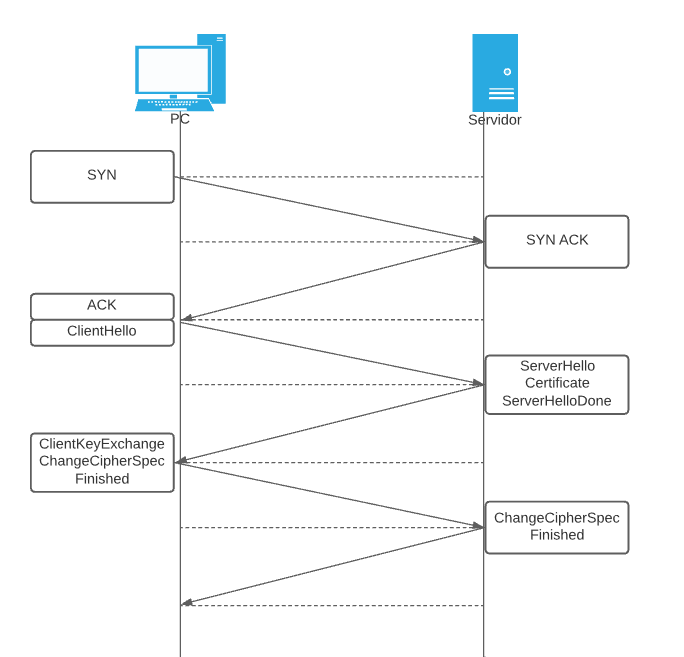
\includegraphics[width=13cm,height=13cm]{2.2.5.png}
      \end{center}
      \caption{Mensajes SSL}
   \end{figure}
\end{center}


\paragraph*{ClientHello}
El mensaje \emph{ClientHello} inicia la comunicación SSL entre las dos partes. 
El cliente usa este mensaje para pedirle al servidor que comience a 
negociar los servicios de seguridad usando SSL.

El mensaje este compuesto por ciertos campos: 
\begin{itemize}
   \setlength\itemsep{-0.6em}
   \item Versión: refiere a la versión más alta de SSL que el cliente 
   puede admitir. 
   \item RandomNumber: proporciona la semilla para cálculos criptográficos
   críticos. 
   \item SessionID: es opcional, y muchas veces no es utilizado. 
   \item CipherSuites: permite a un cliente enumerar los diversos 
   servicios criptográficos que el cliente puede admitir
   \item CompressionMethods: es utilizado por el cliente para enumerar 
   todos los diversos métodos de compresión de datos que puede admitir.
    Los métodos de compresión son una parte importante de SSL porque el 
    cifrado tiene una secuencia significativa en la efectividad de 
    cualquier técnica de compresión de datos. 
\end{itemize}


\paragraph*{ServerHello}
Este mensaje complementa el campo \emph{CipherSuite} del \emph{ServerHello}. Si bien 
el campo \emph{CipherSuite} indica los algoritmos criptográficos y los tamaños 
de clave, este mensaje contiene la información de la clave pública en sí. 
Tenga en cuenta que el mensaje \emph{ServerKeyExchange} se transmite sin cifrado, 
por lo que solo se puede incluir de forma segura información de clave 
pública. El cliente utilizará la clave pública del servidor para cifrar 
una clave de sesión, que las partes utilizarán para cifrar los datos de 
la aplicación para la sesión.

\paragraph*{ServerKeyExchange}

Este mensaje complementa el campo \emph{CipherSuite} del \emph{ServerHello}. 
Si bien el campo \emph{CipherSuite} indica los algoritmos criptográficos y 
los tamaños de clave, este mensaje contiene la información de la clave 
pública en sí. Tenga en cuenta que el mensaje \emph{ServerKeyExchange} se 
transmite sin cifrado, por lo que solo se puede incluir de forma 
segura información de clave pública. El cliente utilizará la clave 
pública del servidor para cifrar una clave de sesión, que las partes 
utilizarán para cifrar los datos de la aplicación para la sesión.

\paragraph*{ServerHelloDone}
El mensaje \emph{ServerHelloDone} le dice al cliente que el servidor ha 
terminado con sus mensajes iniciales de negociación. El mensaje en 
sí no contiene otra información, pero es importante para el cliente, 
porque una vez que el cliente recibe un \emph{ServerHelloDone}, puede pasar a 
la siguiente fase para establecer las comunicaciones seguras.

\paragraph*{ClientKeyExchange}
Cuando el servidor ha terminado su parte de la negociación SSL inicial, 
el cliente responde con un mensaje \emph{ClientKeyExchange}. Así como 
\emph{ServerKeyExchange} proporciona la información clave para el servidor, 
\emph{ClientKeyExchange} le dice al servidor la información clave del cliente. 
En este caso, sin embargo, la información clave es para el algoritmo de 
cifrado simétrico que ambas partes usarán para la sesión. Además, la 
información del mensaje del cliente se cifra mediante la clave pública 
del servidor. Este cifrado protege la información de la clave a medida 
que atraviesa la red y permite al cliente verificar que el servidor 
realmente posee la clave privada correspondiente a su clave pública. 
De lo contrario, el servidor no podrá descifrar este mensaje. Esta 
operación es una protección importante contra un atacante que intercepta 
mensajes de un servidor legítimo y finge ser ese servidor reenviando los 
mensajes a un cliente desprevenido. Dado que un servidor falso no conocerá 
la clave privada del servidor real, no podrá descifrar el mensaje 
\emph{ClientKeyExchange}. Sin la información en ese mensaje, la comunicación 
entre las dos partes no puede tener éxito.
\paragraph*{ChangeCipherSpec}
Una vez que el cliente envía información clave en un mensaje 
\emph{ClientKeyExchange}, se completa la negociación SSL preliminar. En ese 
momento, las partes están listas para comenzar a utilizar los servicios 
de seguridad que han negociado.

El protocolo SSL define un mensaje especial, \emph{ChangeCipherSpec}, para 
indicar explícitamente que ahora se deben invocar los servicios de 
seguridad. Un conjunto de claves protegerá los datos que el cliente 
envía al servidor, y un conjunto diferente de claves protegerá los 
datos que el servidor envía al cliente. Para cualquier sistema dado, 
ya sea un cliente o un servidor, SSL define un estado de escritura y 
un estado de lectura. El estado de escritura define la información de 
seguridad de los datos que envía el sistema y el estado de lectura 
define la información de seguridad de los datos que recibe el sistema.

\paragraph*{Finished}
Inmediatamente después de enviar sus mensajes \emph{ChangeCipherSpec}, cada 
sistema también envía un mensaje \emph{Finished}. Los mensajes \emph{Finished}
permiten que ambos sistemas verifiquen que la negociación se ha realizado 
correctamente y que la seguridad no se ha visto comprometida.

Cada mensaje \emph{Finished} contiene un hash criptográfico de información 
importante sobre la negociación recién finalizada. Esto protege contra 
un atacante que logra insertar mensajes ficticios o eliminar mensajes 
legítimos de la comunicación. Si un atacante pudiera hacerlo, los 
cálculos de hash del cliente y del servidor no coincidirían y detectarían 
el compromiso.

\paragraph*{Finalización de las comunicaciones seguras}

Aunque, en la práctica, rara vez se utiliza (principalmente debido a la 
naturaleza de las sesiones web), SSL tiene un procedimiento definido para 
finalizar una comunicación segura entre dos partes. En este procedimiento, 
los dos sistemas envían cada uno una alerta de cierre especial al otro. 
El cierre explícito de una sesión protege contra un ataque de truncamiento,
en el que un atacante puede comprometer la seguridad al terminar 
prematuramente una comunicación.

\subsubsection*{Autenticar la identidad del servidor}
Anteriormente se explicó cómo SSL puede establecer comunicaciones 
cifradas entre dos partes, lo que puede no agregar mucha seguridad a 
la comunicación. Con el cifrado solo, ninguna de las partes puede 
estar realmente segura de la identidad de la otra. La razón típica 
para usar el cifrado en primer lugar es mantener la información en 
secreto de algún tercero. Pero si ese tercero pudiera hacerse pasar 
con éxito como el destinatario previsto de la información, entonces el 
cifrado no serviría de nada. Los datos estarían encriptados, pero el 
atacante tendría todos los datos necesarios para desencriptarlos. Para 
evitar este tipo de ataques, SSL incluye mecanismos que permiten a cada 
parte autenticar la identidad de la otra. Con estos mecanismos, cada 
parte puede estar segura de que la otra es genuina y no un atacante 
enmascarado. En esta sección, veremos cómo SSL permite que un servidor 
se autentique.

\paragraph*{Certificate}
Al autenticar su identidad, el servidor envía un mensaje de certificado 
en lugar del mensaje \emph{ServerKeyExchange} descrito anteriormente. El mensaje 
\emph{Certificate} simplemente contiene una cadena de certificados que comienza 
con el certificado de clave pública del servidor y termina con el certificado 
raíz de la autoridad certificadora.

El cliente tiene la responsabilidad de asegurarse de que puede confiar 
en el certificado que recibe del servidor. Esa responsabilidad incluye 
verificar las firmas del certificado, los tiempos de validez y el estado 
de revocación. También significa asegurarse de que la autoridad de 
certificación sea una en la que el cliente confíe. Normalmente, los clientes 
toman esta determinación conociendo la clave pública de las autoridades de 
certificación confiables de antemano, a través de algunos medios confiables. 
Microsoft, por ejemplo, carga su software con claves públicas para 
autoridades de certificación conocidas.

\paragraph*{ClientKeyExchange}
El mensaje \emph{ClientKeyExchange} del cliente también difiere en la autenticación 
del servidor, aunque la diferencia no es importante. Cuando solo se va a 
utilizar cifrado, el cliente cifra la información en en mensaje 
\emph{ClientKeyExchange}
utilizando la clave pública que el servidor proporciona en su mensaje 
\emph{ServerKeyExchange}. En este caso, por supuesto, el servidor se está 
autenticando y, por lo tanto, ha enviado un mensaje de certificado en 
lugar de un \emph{ServerKeyExchange}. El cliente, por lo tanto, encripta su 
información usando la clave pública contenida en el 
certificado del servidor. Este paso es importante porque le permite 
al cliente asegurarse de que la parte con la que se está comunicando 
realmente posee la clave privada del servidor. Solo un sistema con la 
clave privada real podrá descifrar este mensaje y continuar con éxito 
la comunicación.

 

\subsubsection*{Niveles de validación}  
Hay tres tipos de certificados SSL disponibles en la actualidad: validación por 
dominio (DV),
validación por organización (OV) y validación extendida (EV).
Los niveles de cifrado son los mismos para cada certificado, lo que difiere son los 
procesos de investigación y verificación necesarios para obtener el certificado.

\paragraph*{Validación de dominio (DV)}
Validación de dominio SSL o DV SSL representa el nivel base para los tipos de SSL. 
Estos son perfectos para sitios web que solo necesitan cifrado y nada más. Los 
certificados DV SSL suelen ser económicos y se pueden emitir en cuestión de minutos. 
Eso es porque el proceso de validación está completamente automatizado. Simplemente 
es necesario demostrar que es propietario de su dominio y que el certificado DV 
es suyo. 

\begin{center}
   \begin{figure}   
      \begin{center}
         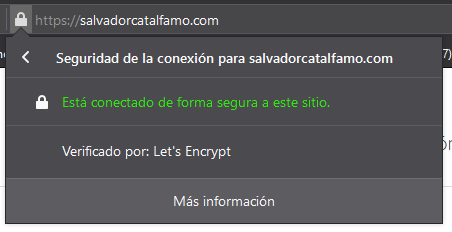
\includegraphics{dv.png}
      \end{center}
      \caption{Validación de dominio}
   \end{figure}
\end{center}

\paragraph*{Validación de la organización (OV)}
Validación de organización u OV SSL representa el término medio para los tipos de 
certificados SSL. Para obtener OV SSL, su empresa u organización debe someterse a 
un examen comercial ligero. Esto puede demorar hasta tres días hábiles porque alguien 
tiene que verificar la información de su empresa. OV SSL muestra los mismos indicadores 
visuales que DV SSL, pero proporciona una forma de ver la 
información comercial verificada en la sección de detalles del certificado. 

\paragraph*{Extended Validation (EV)}
SSL de validación extendida o SSL con EV requiere un exhaustivo examen comercial. 
Esto puede parecer mucho, pero en realidad no lo es si su empresa tiene 
registros disponibles públicamente. EV SSL activaba un indicador visual único: el 
nombre de su organización verificado que se muestra en el navegador. Esto en la 
actualidad ya no sucede, por lo que no es posible a simple vista identificarlo.

\begin{center}
   \begin{figure}   
      \begin{center}
         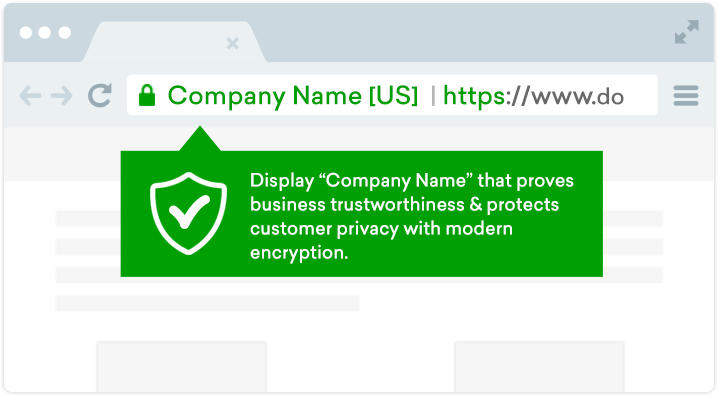
\includegraphics[width=11cm,height=6.5cm]{ev.png}
      \end{center}
      \caption{Validación extendida (Captura antigua)}
   \end{figure}
\end{center}

  \subsubsection*{Tipos de certificados}

  \paragraph*{Dominio Simple}
  Como sugiere el nombre, un certificado SSL de un solo dominio solo 
  se puede usar en un solo dominio o IP. Este se considera el tipo de 
  certificado SSL predeterminado. 
  
  \paragraph*{Multi-Dominio}
  Este tipo de SSL es un certificado para todos los usos. Permiten cifrar 
  hasta 250 dominios diferentes y subdominios 
  ilimitados. Desafortunadamente, no está disponible en EV.
  
  \paragraph*{Wildcard}
  
  Los \emph{wildcard} están diseñados específicamente para cifrar un dominio y 
  todos los subdominios que lo acompañan (también representado como *.dominio.com). 
  Desafortunadamente, los \emph{wildcard} solo están disponibles en los 
  niveles DV y OV.
  
  \paragraph*{Multi-Dominio Wildcard}
  Los \emph{wildcard} multidominio pueden cifrar hasta 250 dominios diferentes 
  y subdominios ilimitados. Desafortunadamente, no está disponible en EV.

  
\subsubsection*{Validación de propiedad de dominio}

Los certificados se utilizan con mayor frecuencia para autenticar 
nombres de dominio. Por lo tanto, se confía en las autoridades de 
certificación (CA) para verificar que un solicitante de un certificado 
represente legítimamente el nombre de dominio en el certificado.

Los diferentes tipos de certificados reflejan diferentes tipos de 
verificación de CA. Los certificados de “Validación de dominio” (DV) son 
el tipo más común. La única validación que debe realizar la CA en el 
proceso de emisión de un certificado DV es verificar que el solicitante 
tiene un control efectivo del dominio. La CA no está obligada a intentar 
verificar la identidad real del solicitante. Esto difiere en los certificados 
de “Validación de la organización” y “Validación extendida”, 
donde el proceso está destinado a verificar también la identidad real del 
solicitante.

ACME (\emph{Automatic Certificate Management Environment})
permite a un cliente 
la automatización de gestión de certificados 
mediante un conjunto de mensajes transmitidos a través de HTTPS. La 
emisión de certificados mediante el protocolo ACME se asemeja al proceso 
de emisión de una CA tradicional, en el que un usuario crea una cuenta, 
solicita un certificado y demuestra el control de los dominios con el 
certificado para que la CA emita el certificado solicitado.


ACME utiliza un \emph{framework} de desafío/respuesta extensible para la validación 
de dominios. El servidor envía al cliente un conjunto de desafíos, y el cliente 
responde enviando la respuesta al mismo en una solicitud POST a una URL de desafío.

Los diferentes desafíos permiten al servidor obtener pruebas de diferentes 
aspectos del control sobre un dominio. En los desafíos como HTTP y 
DNS, el cliente demuestra directamente su capacidad para hacer ciertas 
acciones relacionadas con el dominio. Es de gran utilidad explicar los 
diferentes tipos de desafíos que se puede ofrecer a un cliente, ya que uno 
es el mas común, sin embargo, al hablar de redes internas, no lo podremos 
utilizar, e iremos por la otra opción, un tanto menos conocida.


\paragraph*{Desafío HTTP}

Con la validación HTTP, el cliente prueba su control sobre un nombre de dominio al 
demostrar que puede guardar recursos HTTP en un servidor accesible bajo ese nombre 
de dominio. El servidor ACME desafía al cliente solicitándole un archivo en una ruta 
específica, con una cadena específica como contenido.

Este es el tipo de desafío más común en la actualidad. El servidor le da un token 
a su cliente ACME y su cliente ACME coloca un archivo en su servidor web 
en {http://\<SU\_DOMINIO\>/.well-known/acme-challenge/\<TOKEN\>}. Ese archivo contiene 
el token, más una huella digital de la clave de su cuenta.

Una vez que el cliente le dice al servidor que el archivo está listo, el servidor 
intenta recuperarlo. Al recibir una respuesta, el servidor construye y almacena la 
autorización de la clave a partir del valor del “token” de desafío y la clave de 
la cuenta del cliente actual.

Dado un par de desafío/respuesta, el servidor verifica el control del dominio por 
parte del cliente verificando que el recurso se aprovisionó como se esperaba.

Ventajas:
\begin{itemize}
   \setlength\itemsep{-0.6em}
   \item Es fácil de automatizar sin conocimientos adicionales sobre la configuración de un dominio.
   \item Funciona con servidores web estándar.
\end{itemize}

Desventajas:
\begin{itemize}
   \setlength\itemsep{-0.6em}
   \item No funciona si su ISP bloquea el puerto 80 (esto es raro, pero algunos ISP residenciales lo hacen).
   \item Let's Encrypt no le permite utilizar este desafío para emitir certificados Wildcard.
   \item Si tiene varios servidores web, debe asegurarse de que el archivo esté disponible en todos ellos.
\end{itemize}
   
Este desafío está fuera de nuestro alcance, ya que partimos de la premisa de que 
el tráfico que queremos proteger nunca saldrá a Internet, lo que implica que no 
tendremos ni puertos ni direcciones expuestas para que un servidor externo pueda 
verificar el recurso mencionado anteriormente. 


\paragraph*{Desafío DNS}
Cuando el identificador que se está validando es un nombre de dominio, el cliente 
puede demostrar el control de ese dominio proporcionando un registro DNS de tipo 
TXT que contenga un valor designado.

Un cliente cumple este desafío construyendo una clave de autorización a partir del 
valor de un token proporcionado y la clave de la cuenta del cliente. A continuación, el 
cliente calcula un hash SHA-256 de la clave de 
autorización.
El registro proporcionado al DNS contiene la codificación de URL base64 de este 
hash. 

\noindent Ejemplo:

Si se desea validar el nombre de dominio “www.ejemplo.org”, el cliente 
proporcionaría el siguiente registro DNS:

\begin{verbatim}
   _acme-challenge.www.ejemplo.org: "gfj9Xq...Rg85nM"
\end{verbatim}

Al recibir una respuesta, el servidor construye y almacena la llave de autorización
clave a partir del valor del “token” del desafío y la clave de la cuenta del cliente actual.

\noindent Para validar un desafío de DNS, el servidor realiza los siguientes pasos:

\begin{enumerate}
   \setlength\itemsep{-0.6em}
   \item Calcula el hash SHA-256 de la clave de autorización almacenada.
   \item Consulta los registros TXT para el nombre de dominio de validación.
   \item Verifica que el contenido de uno de los registros TXT coincida con el valor de hash.
\end{enumerate}

   
Si todas las verificaciones anteriores tienen éxito, entonces la validación es exitosa. 
Si no se encuentra ningún registro DNS, o si el registro DNS y el contenido del mismo 
no pasan estas comprobaciones, la validación falla.